% THIS IS SIGPROC-SP.TEX - VERSION 3.1
% WORKS WITH V3.2SP OF ACM_PROC_ARTICLE-SP.CLS
% APRIL 2009
%
% It is an example file showing how to use the 'acm_proc_article-sp.cls' V3.2SP
% LaTeX2e document class file for Conference Proceedings submissions.
% ----------------------------------------------------------------------------------------------------------------
% This .tex file (and associated .cls V3.2SP) *DOES NOT* produce:
%       1) The Permission Statement
%       2) The Conference (location) Info information
%       3) The Copyright Line with ACM data
%       4) Page numbering
% ---------------------------------------------------------------------------------------------------------------
% It is an example which *does* use the .bib file (from which the .bbl file
% is produced).
% REMEMBER HOWEVER: After having produced the .bbl file,
% and prior to final submission,
% you need to 'insert'  your .bbl file into your source .tex file so as to provide
% ONE 'self-contained' source file.
%
% Questions regarding SIGS should be sent to
% Adrienne Griscti ---> griscti@acm.org
%
% Questions/suggestions regarding the guidelines, .tex and .cls files, etc. to
% Gerald Murray ---> murray@hq.acm.org
%
% For tracking purposes - this is V3.1SP - APRIL 2009

\documentclass{acm_proc_article-sp}

\usepackage{url}
\usepackage{natbib}

\begin{document}

\title{Improving Data Collection and Monitoring through Dynamic Data Analysis}
\subtitle{}
%
% You need the command \numberofauthors to handle the 'placement
% and alignment' of the authors beneath the title.
%
% For aesthetic reasons, we recommend 'three authors at a time'
% i.e. three 'name/affiliation blocks' be placed beneath the title.
%
% NOTE: You are NOT restricted in how many 'rows' of
% "name/affiliations" may appear. We just ask that you restrict
% the number of 'columns' to three.
%
% Because of the available 'opening page real-estate'
% we ask you to refrain from putting more than six authors
% (two rows with three columns) beneath the article title.
% More than six makes the first-page appear very cluttered indeed.
%
% Use the \alignauthor commands to handle the names
% and affiliations for an 'aesthetic maximum' of six authors.
% Add names, affiliations, addresses for
% the seventh etc. author(s) as the argument for the
% \additionalauthors command.
% These 'additional authors' will be output/set for you
% without further effort on your part as the last section in
% the body of your article BEFORE References or any Appendices.

\numberofauthors{1} %  in this sample file, there are a *total*
% of EIGHT authors. SIX appear on the 'first-page' (for formatting
% reasons) and the remaining two appear in the \additionalauthors section.
%
\author{
% You can go ahead and credit any number of authors here,
% e.g. one 'row of three' or two rows (consisting of one row of three
% and a second row of one, two or three).
%
% The command \alignauthor (no curly braces needed) should
% precede each author name, affiliation/snail-mail address and
% e-mail address. Additionally, tag each line of
% affiliation/address with \affaddr, and tag the
% e-mail address with \email.
%
\alignauthor
P. Lubell-Doughtie, P. Pokharel, M. Johnston, V. Modi\\
       \affaddr{Columbia University}\\
       \affaddr{New York, New York}\\
       \email{\{pl2472, pp2427, mj2537, modi\}@columbia.edu}
}
% Just remember to make sure that the TOTAL number of authors
% is the number that will appear on the first page PLUS the
% number that will appear in the \additionalauthors section.

\maketitle
\begin{abstract}
Feedback based on real-time data is increasingly important for ICT-based interventions in the developing world. Applications such as 
facility inventories,
summarization of patient data from community health workers, 
etc. need processes for analyzing and aggregating datasets that update over time. In order to facilitate such processes, we have created a modular web service for real-time data analysis: Bamboo.
\end{abstract}

% A category with the (minimum) three required fields
%\category{H.4}{Information Systems Applications}{Miscellaneous}
%A category including the fourth, optional field follows...
%\category{D.2.8}{Software Engineering}{Metrics}[complexity measures, performance measures]

%\terms{Theory}

%\keywords{ACM proceedings, \LaTeX, text tagging} % NOT required for Proceedings

\section{Introduction}
In order to effectively monitor community health, allocate resources, and respond to crises, both countries and planners need real-time data. 
To address this, tools like EpiSurveyor, OpenDataKit, and formhub.org allow development planners and others to conduct data gathering exercises without the need for server infrastructure or in-house programmers.  
But, data collection is only part of the picture.

In emergency response, the time lag in processing of structured data causes significant delays; faster data analysis allows decision makers to address problems sooner and have a greater impact \cite{internews}.
Health workers and managers can learn how to best to modify their health programs
and avert future deaths
through access to audit trails based on timely data \cite{krisberg}.
In mobile health systems, monitoring real-time reports can improve health programs and address key health risks \cite{mechael}.  

Dynamic data analysis, a prerequisite for such applications, demands resources and skills that are often unavailable in the development context.  Even simplistic systems that perform user-defined aggregations and calculations on dynamic datasets require high technical capacity.  Bamboo provides real-time aggregation, calculation, and summarization as a hosted web service.\footnote{\url{http://bamboo.io/}}  Practitioners can interact with Bamboo using an easy to learn syntax.

Before building Bamboo, we categorized existing solutions for dynamic data analysis as: custom tools, hosted tools, and offline tools.  Custom tools are either built in-house or by a third-party, which are expensive and often beyond the capacity of most organizations. Furthermore, custom tools often lead to duplication of effort and are difficult to adapt to new tasks.  Popular hosted tools, such as Google Fusion Tables and Google Docs, had functional limitations that prevented their use.  Google Fusion Tables only allows a limited set of calculations, and the ``one spreadsheet'' model of Google Docs precludes aggregations \cite{gonzalez1, gonzalez2}.  Offline data analysis tools, Microsoft Excel, Python, R, SPSS, STATA, etc. have the flexibility required but have steep learning curves and require programmatic wrappers to allow for truly dynamic workflows, creating high barriers to entry.

\section{Design}

\begin{figure}
\centering
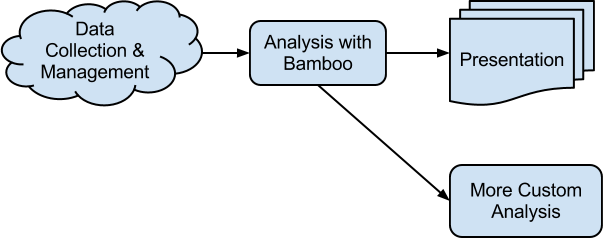
\includegraphics[width=3in]{figures/bamboo_flow}
\caption{Systematizing data collection and reporting with Bamboo.}
\label{fig:flow}
\end{figure}

Bamboo sits between data collection and reporting, Fig. \ref{fig:flow}. The
dynamic statistical analysis within bamboo allows practitioners to easily build
dashboards, maps, and tables; which automatically update as new data
arrives.  This enables the split-apply-combine strategy of data analysis
\cite{wickham} through a web service.  
Bamboo's core functionality allows
practitioners to: (1) store, update, and merge datasets, (2) build algebraic calculations and aggregations, and (3) generate summary statistics, means, counts, etc.

Generalizability is a fundamental principle of the design: Bamboo accepts any
CSV file and provides users with complete control of their calculations.
Updates are triggered programmatically with a simple JSON web request, making it
very easy to link data from a variety of sources.
These updates are propagated through the system ensuring that any aggregations or merged datasets are synchronized with the most recent data, as shown in Fig. \ref{fig:updates}.  
We have integrated automatic updates to the Bamboo web service from our mobile data collection platform, formhub.org.

To encourage community use and development we have made Bamboo open source and structured it to be easily extendable.  We also offer Bamboo as a hosted web service.  The Bamboo web service uses REST conventions and we have built client libraries that communicate with it in Python and JavaScript.  For numerical computation Bamboo uses the high-performance statistical package pandas \cite{mckinney}.

\begin{figure}
\centering
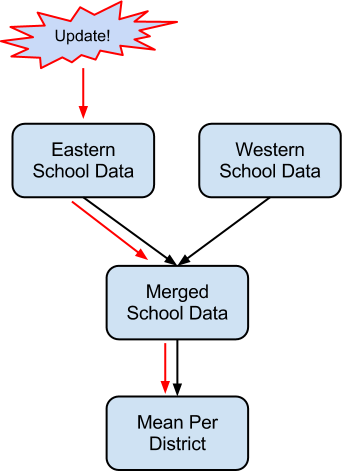
\includegraphics[width=2in]{figures/update_flow}
\caption{An update propagates from the dataset to all downstream merged datasets and aggregations.  The black arrows show structural dependencies created by the client.  The red arrow shows an update propagating through the system.}
\label{fig:updates}
\end{figure}

\section{Case Study}

\begin{figure}
\centering
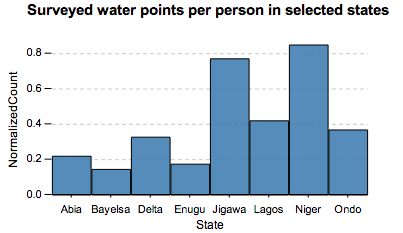
\includegraphics[width=3.5in]{figures/summary.png}
\caption{After merging datasets, the normalization formula required one API call to establish. Thereafter, the same URL provides updated data to produce the graph above at any point in the survey process.}
\label{fig:summary}
\end{figure}

During a large data collection project in Nigeria, researchers used Bamboo to monitor the progress of a public water facilities survey as it was conducted across the country. By summarizing the amount of data collected per state, data collection monitors were able to identify states in which data coverage was lower than expected.
Bamboo also allowed researchers to conduct exploratory monitoring of this
dataset using complex metrics, such as number of waterpoints surveyed per 1000
people, presented in Fig. \ref{fig:summary}.

%\section{Discussion}

%Fig. \ref{fig:berg} shows a truncated version of a Community Health Worker 30 day performance monitoring table used in the ChildCount+ system \cite{berg}.  The ability to create and review this information was a crucial component of a larger system for improving the registration of children and ultimately health interventions, such as immunizations and monitoring risk factors.
%
%By connecting the ChildCount+ data collection infrastructure to Bamboo, practitioners are provided with the statistical analysis needed to build this table in \emph{real-time} as more data arrives.  Requiring only a minimal amount of effort and expertise, what were formerly static reports or charts can become dynamic monitor tools.
%
%\begin{figure}
%\centering
%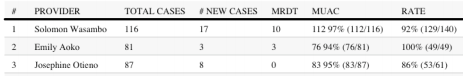
\includegraphics[width=3.5in]{figures/berg_table}
%\caption{A Community Health Worker 30 day performance monitoring table\cite{berg}.}
%\label{fig:berg}
%\end{figure}

\section{Conclusions and Future Work}
Bamboo allows users without programming expertise to do dynamic data analysis.  Bamboo systematizes the process of creating indicators for domain specific data sets thereby reducing the time between collection and analysis, as well as the time between analysis and reporting.
We see immediate application in the development context, making performance monitoring \cite{berg} and real-time outlier detection in categorical data \cite{dimagi} much easier to implement. 

In the future we will add additional analysis tools to encompass more real-world data processing tasks, such as levenshtein distance, nearest neighbors using k-means, time series analysis, and spatial analysis.  We plan to offer ``calculation libraries'' and allows users to build a set of calculations---e.g. health indicators---once, and then apply the same calculations to many datasets.

%\end{document}  % This is where a 'short' article might terminate

%
% The following two commands are all you need in the
% initial runs of your .tex file to
% produce the bibliography for the citations in your paper.
\bibliographystyle{abbrv}
\bibliography{acm_dev2013_mrg}  % sigproc.bib is the name of the Bibliography in this case
% You must have a proper ".bib" file
%  and remember to run:
% latex bibtex latex latex
% to resolve all references
%
% ACM needs 'a single self-contained file'!
%
%APPENDICES are optional
%\balancecolumns

\balancecolumns
% That's all folks!
\end{document}
